\documentclass[conference]{IEEEtran}
\usepackage{graphicx}
\usepackage{booktabs}
\usepackage{amsmath}
\usepackage{url}
\usepackage{cite}
\usepackage[hidelinks]{hyperref}

\begin{document}

\title{Name Games: Adversarial Domain Renaming Against Machine Learning Phishing Detectors}

\author{\IEEEauthorblockN{Aakash Tiwari}
\IEEEauthorblockA{Rowan University\\
Glassboro, NJ, USA}}

\maketitle

\begin{abstract}
Machine learning models that flag phishing links from the host name alone are attractive for settings such as QR code scanning, where a decision must be made before a page is opened. However, every character such a model sees is chosen by the attacker. We study how cheaply an attacker can rename a phishing host to evade these models. We define seven realistic renaming edits, including swapping the top-level domain, adding a benign word, and removing hyphens, digits or alarming keywords, under constraints that keep the brand being imitated and forbid hosts the attacker could not register. On the PhiUSIIL dataset with a domain-grouped split, a black-box attacker that queries the model about 34 times evades a blend of XGBoost and character n-gram classifiers for 48.5\% of detected phishing hosts with a single edit and 83.9\% with four edits, while random edits succeed only 10.1\% of the time. Swapping the top-level domain to a common one such as \texttt{.com} or \texttt{.org} alone evades 44.7\%. Adversarial training with two rounds of attack-generated hosts lowers four-edit evasion against an adaptive attacker using unseen words to 51.3\% and nearly triples recall under attack, from 10.7\% to 29.7\%, with no loss in clean recall at a fixed 5\% false alarm rate. The defense has a cost: more renamed legitimate hosts are flagged. Our results show that host-only phishing detectors should be treated as a cheap first filter and paired with signals the attacker cannot rename.
\end{abstract}

\begin{IEEEkeywords}
phishing detection, adversarial machine learning, URL classification, adversarial training, quishing
\end{IEEEkeywords}

\section{Introduction}

Phishing remains one of the most common entry points for fraud and account takeover. A large body of work trains classifiers on URLs to flag phishing links before a user visits them \cite{ma2009beyond, sahoo2017survey, le2018urlnet, bahnsen2017rnn}. Lexical models are fast, need no network access, and can run on a phone, which makes them a natural fit for QR code phishing (``quishing''), where a code on a poster or parking meter hides its destination until the user opens it \cite{trad2025quishing}.

While building a QR code scanner, we found that the widely used PhiUSIIL dataset \cite{prasad2024phiusiil} contains a strong shortcut: every legitimate URL is a bare homepage, so a model given the full URL learns that any path means phishing. We therefore built a detector that sees only the host name, evaluated on websites never seen during training. This removes the shortcut, but it raises a different question. The host name is exactly the part of a URL that a phishing operator chooses when registering a domain. If a model relies on cheap choices such as the top-level domain (TLD), the attacker can simply make a different choice.

This paper asks how easily an attacker can rename a phishing host to evade a host-based detector, and whether retraining on renamed hosts helps. Unlike attacks that perturb feature vectors or embeddings, we work in the problem space \cite{pierazzi2020problemspace}: every adversarial example is a valid host name that an attacker could plausibly register, which keeps the brand being imitated and does not take over an existing legitimate domain. Our contributions are:

\begin{itemize}
\item A threat model and seven renaming edits for host names, with realism constraints, and a simple query-based greedy attack.
\item An evaluation on 39,454 test URLs from unseen domains showing that a blended detector is evaded for 83.9\% of detected phishing hosts within four edits and about 34 queries, and that a TLD swap alone evades 44.7\%.
\item An analysis of which edits work, how attacks transfer between model types, and why random renaming is a misleading measure of robustness.
\item An adversarial training study with an adaptive attacker that uses words never seen in training, showing a clear but partial gain in robustness and its cost in false alarms on renamed legitimate hosts.
\end{itemize}

\section{Background and Related Work}

\textbf{URL-based phishing detection.} Ma et al.\ showed that lexical and host features of URLs can separate malicious from benign sites \cite{ma2009beyond}. Later work used character-level recurrent and convolutional networks \cite{bahnsen2017rnn, le2018urlnet}; Sahoo et al.\ survey the area \cite{sahoo2017survey}. PhiUSIIL \cite{prasad2024phiusiil} is a recent dataset of 235,795 URLs with URL and page features. Arp et al.\ list common pitfalls in security machine learning, including sampling bias and spurious correlations \cite{arp2022dos}, which match the shortcut we found in PhiUSIIL and connect to the broader problem of shortcut learning \cite{geirhos2020shortcut}.

\textbf{Adversarial machine learning.} Small, targeted changes to inputs can fool classifiers \cite{goodfellow2015explaining, biggio2018wild}, and adversarial training is the standard empirical defense \cite{madry2018towards}. In security, Pierazzi et al.\ argue that attacks must produce real, valid objects rather than arbitrary feature vectors \cite{pierazzi2020problemspace}, and Apruzzese et al.\ note that real attackers rarely compute gradients and instead use cheap, black-box changes \cite{apruzzese2023real}. Our attack follows this view: it uses only model scores and edits that a domain registrant can make.

\textbf{Attacks on phishing detectors.} Shirazi et al.\ showed that phishing detectors based on hand-crafted features can be evaded by sampling feature values \cite{shirazi2019adversarial}, and AlEroud and Karabatis generated evasive URLs with generative adversarial networks \cite{aleroud2020bypassing}. Our edits are deliberately simpler and grounded in known domain abuse: combosquatting, where a brand is combined with other words \cite{kintis2017combosquatting}, and homograph attacks, which swap visually similar characters \cite{holgers2006homograph}. We focus on host-only models, which matter for pre-visit settings such as QR scanning, and we evaluate defenses against an adaptive attacker.

\section{Threat Model}

\textbf{Target.} A binary classifier assigns a phishing score to a host name, and the host is flagged when the score is at or above a threshold. The path and query string are ignored, which avoids the PhiUSIIL shortcut.

\textbf{Attacker goal.} Starting from a phishing host that the model detects, produce a renamed host that the model does not flag, while keeping the host useful for phishing.

\textbf{Attacker knowledge.} We consider (i) a \emph{query} attacker who can submit candidate hosts and read the score, as with a public scanning app or API, and (ii) a \emph{random} attacker who applies edits without any queries. We also measure transfer from a surrogate model to a different target.

\textbf{Attacker capabilities.} The attacker controls the host they register: the second-level name, the TLD among common choices, and subdomain labels under their own domain. Each candidate host must satisfy the following constraints:
\begin{enumerate}
\item It is valid DNS syntax and is not an IP address.
\item Every brand name in the original host, written plainly or with look-alike characters, is still present.
\item Its registered domain is not one of the legitimate registered domains in the dataset, since those are already owned.
\item It does not reduce a host that had subdomains to the bare registered domain, because many such hosts live under shared services where the attacker controls only a subdomain.
\end{enumerate}
The attacker may apply up to $k$ edits, which we call the edit budget.

\section{Renaming Edits and Attacks}

\subsection{Edits}
Table~\ref{tab:edits} lists the seven edits. Each is something phishing operators already do or could do for a few dollars. Removing a keyword such as \texttt{login} does not remove it from the attack, since the word can move to the URL path, which the model ignores.

\begin{table}[t]
\centering
\caption{Renaming edits used by the attacker}
\label{tab:edits}
\footnotesize
\setlength{\tabcolsep}{3pt}
\begin{tabular}{@{}ll@{}}
\toprule
Edit & Example \\
\midrule
TLD swap & \texttt{sgpay.top} $\rightarrow$ \texttt{sgpay.org} \\
Benign word & \texttt{metamaskdesk.com} $\rightarrow$ \texttt{metamaskdeskcity.com} \\
Digit removal & \texttt{pay24bank.xyz} $\rightarrow$ \texttt{paybank.xyz} \\
Hyphen removal & \texttt{iran-peygiri.ml} $\rightarrow$ \texttt{iranpeygiri.ml} \\
Keyword removal & \texttt{login-nab-au.com} $\rightarrow$ \texttt{nab-au.com} \\
Homoglyph & \texttt{account} $\rightarrow$ \texttt{acc0unt} \\
Subdomain strip & \texttt{a.b.evil.xyz} $\rightarrow$ \texttt{b.evil.xyz} \\
\bottomrule
\end{tabular}
\end{table}

TLD swaps use \texttt{.com}, \texttt{.net}, \texttt{.org}, \texttt{.io}, \texttt{.co} and \texttt{.us}. Benign words are added at the start or end of the second-level name. We use two disjoint lists of 12 common words: a training list (for example \texttt{online}, \texttt{shop}, \texttt{news}) used only by the defender, and a test list (for example \texttt{cloud}, \texttt{tech}, \texttt{blog}) used only by the attacker during evaluation. This prevents a defense from simply memorizing the attacker's vocabulary.

\subsection{Attacks}
The \textbf{greedy query attack} starts from the original host. At each step it generates every valid single-edit candidate of the current host, queries all of them, and keeps the one with the lowest score. It stops when the score falls below the threshold or the budget $k$ is reached. The \textbf{random attack} picks a valid candidate uniformly at random at each step and never queries the model. The greedy attack is not optimal, so its success rate is a lower bound on what a stronger attacker could achieve.

\section{Experimental Setup}

\textbf{Data.} We use the PhiUSIIL dataset \cite{prasad2024phiusiil}, flipping its labels so that 1 means phishing. After removing duplicate URLs, 235,370 remain. We drop URLs on link shorteners, shared services (such as Google Docs) and free hosting platforms, where the host name alone cannot judge a page, leaving 204,989 URLs. We split by registered domain, so that every website appears in only one part: 148,868 training, 16,667 validation and 39,454 test URLs. Each URL is reduced to its lower-cased host without \texttt{www.}.

\textbf{Models.} Following our QR scanner, we use three models: (i) XGBoost \cite{chen2016xgboost} with 400 trees on 48 hand-made host features, such as lengths, digit and hyphen counts, entropy, subdomain depth, brand and keyword indicators, look-alike characters and one-hot TLDs; (ii) logistic regression on TF-IDF character n-grams of length 2 to 5; and (iii) a blend that averages the two scores. For each model, the threshold is set on legitimate validation hosts to give a 5\% false alarm rate.

\textbf{Attack set.} The test set contains 10,707 unique phishing hosts that are not IP addresses. Of these, the XGBoost, n-gram and blend models detect 5,179, 6,597 and 6,498 respectively. For each model we attack a random sample of 1,500 detected hosts.

\textbf{Metrics.} The \emph{evasion rate} is the share of attacked hosts whose renamed version is no longer flagged. For defenses we also report clean ROC AUC, recall and false alarm rate on all test URLs, and an estimate of \emph{recall under attack}, the clean recall multiplied by one minus the four-edit evasion rate.

\section{Results}

\subsection{How vulnerable are host-based detectors?}

Table~\ref{tab:clean} shows clean performance. The n-gram model and the blend rank hosts similarly well, and all models catch 49--62\% of phishing URLs on unseen domains at about 5\% false alarms.

\begin{table}[t]
\centering
\caption{Clean test performance at a 5\% validation false alarm rate}
\label{tab:clean}
\begin{tabular}{@{}lccc@{}}
\toprule
Model & ROC AUC & Recall & False alarms \\
\midrule
XGBoost (48 features) & 0.816 & 49.4\% & 4.2\% \\
Character n-grams & 0.877 & 62.5\% & 4.9\% \\
Blend & 0.875 & 61.5\% & 4.3\% \\
\bottomrule
\end{tabular}
\end{table}

Fig.~\ref{fig:budget} shows evasion as the edit budget grows. A single edit evades 47.5\% of detected hosts for XGBoost, 59.1\% for the n-gram model and 48.5\% for the blend. With four edits, evasion reaches 75.1\%, 95.2\% and 83.9\%. A successful evasion needed a median of only 34, 33 and 34 queries. The blend is more robust than the n-gram model alone, but it does not stop a patient attacker.

Random edits are far weaker. With four random edits, only 10.1\% of hosts evade the blend, and the rate does not grow with the budget, because random edits are as likely to make a host look worse as better. Robustness measured with random perturbations would therefore give a false sense of security; the meaningful threat is an attacker who can test candidates.

\begin{figure}[t]
\centering
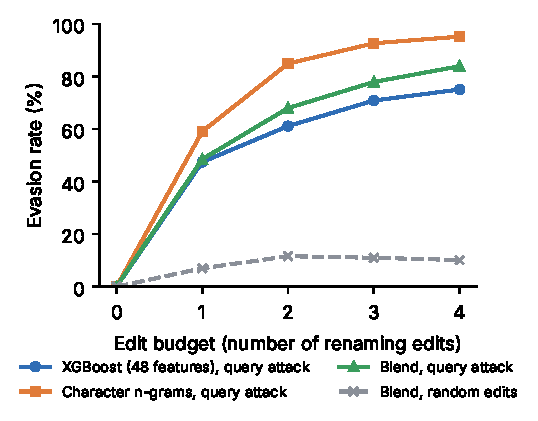
\includegraphics[width=\columnwidth]{evasion_budget.pdf}
\caption{Share of detected phishing hosts that evade each model as the number of renaming edits grows. Query attacks use the model's score; random edits do not.}
\label{fig:budget}
\end{figure}

\subsection{Which edits work?}

Fig.~\ref{fig:single} restricts the attacker to one edit type and one step against the blend. Swapping the TLD alone evades 44.7\% of detected hosts. Every host can receive this edit, and a \texttt{.com} or \texttt{.org} name costs the attacker only a few dollars more than \texttt{.xyz} or \texttt{.top}. Adding a benign word evades 15.7\%. Removing a keyword works for 29.2\% of the hosts that contain one, but only 5.9\% of hosts do. Homoglyphs barely help (1.2\%), since look-alike digits are themselves a strong phishing signal, and stripping one subdomain level never evaded the blend.

Among the 1,259 hosts that evaded the blend within four edits, TLD swaps made up 54\% of all edits used (1,135 of 2,119), followed by benign words (373) and digit removal (301). The models have learned that cheap TLDs are suspicious, which is true in the data, but it is a feature the attacker controls completely. Fig.~\ref{fig:examples} gives examples.

\begin{figure}[t]
\centering
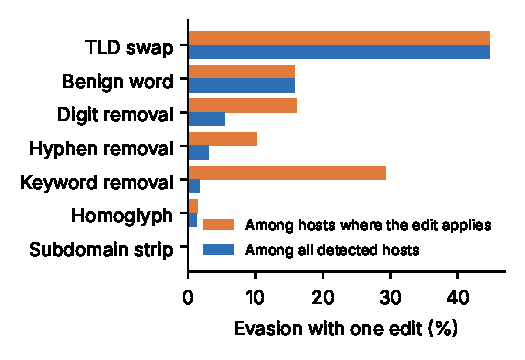
\includegraphics[width=\columnwidth]{single_edit.pdf}
\caption{Evasion of the blend with a single edit of one type. Blue: share of all detected hosts. Orange: share of hosts where that edit can be applied.}
\label{fig:single}
\end{figure}

\begin{figure}[t]
\centering
\footnotesize
\begin{tabular}{@{}ll@{}}
\toprule
Original (flagged) & Renamed (not flagged) \\
\midrule
\texttt{sadad-shaparak.cf} & \texttt{sadad-shaparak.org} \\
\texttt{caderastreamento.com.br} & \texttt{caderastreamento.org} \\
\texttt{iran-peygiri.ml} & \texttt{iran-peygiri.org} \\
\texttt{confirm-profile-nab.com} & \texttt{profile-nab.org} \\
\texttt{metamaskdesk.com} & \texttt{metamaskdeskcity.org} \\
\texttt{yoindomin-irs.ml} & \texttt{yoindominirs.org} \\
\bottomrule
\end{tabular}
\caption{Phishing hosts from the test set and the renamed versions that evade the blend, found by the greedy attack.}
\label{fig:examples}
\end{figure}

\subsection{Do attacks transfer?}

Table~\ref{tab:transfer} shows how often a host renamed to evade one model also evades another model that originally detected it. Attacks crafted against the blend transfer well to its two parts (81.1\% and 86.5\%), while attacks against a single model transfer less (45.1\% to 69.3\%). An attacker without query access could therefore build a local blend as a surrogate and still succeed most of the time.

\begin{table}[t]
\centering
\caption{Transfer of successful renamings (rows: model attacked; columns: model tested)}
\label{tab:transfer}
\begin{tabular}{@{}lccc@{}}
\toprule
Crafted against & XGBoost & n-grams & Blend \\
\midrule
XGBoost & -- & 57.6\% & 69.3\% \\
n-grams & 45.1\% & -- & 59.9\% \\
Blend & 81.1\% & 86.5\% & -- \\
\bottomrule
\end{tabular}
\end{table}

\subsection{Does adversarial training help?}

We compare four ways of training the blend. \emph{Standard} uses only the training data. \emph{Random renaming} adds 10,000 training phishing hosts, each renamed with one to three random edits. \emph{Adversarial (1 round)} instead adds the hosts produced by running the greedy attack against the standard blend on the same 10,000 training hosts. \emph{Adversarial (2 rounds)} then attacks the 1-round model on another 10,000 training hosts and retrains with both sets. All added hosts are labeled phishing and use the training word list. Every model is recalibrated to a 5\% validation false alarm rate and then attacked by a fresh greedy attacker that uses the unseen test word list. Table~\ref{tab:defense} and Fig.~\ref{fig:defense} show the results. The standard model is attacked on a new sample here, so its evasion rate (82.5\%) differs slightly from Fig.~\ref{fig:budget}.

\begin{table}[t]
\centering
\caption{Defenses against an adaptive greedy attacker with unseen words}
\label{tab:defense}
\setlength{\tabcolsep}{3.5pt}
\begin{tabular}{@{}lccccc@{}}
\toprule
Training & AUC & Recall & \multicolumn{2}{c}{Evasion} & Recall under \\
 & & & 1 edit & 4 edits & attack \\
\midrule
Standard & 0.875 & 61.5\% & 47.9\% & 82.5\% & 10.7\% \\
Random renaming & 0.871 & 61.3\% & 45.4\% & 69.8\% & 18.5\% \\
Adversarial, 1 round & 0.858 & 61.0\% & 37.4\% & 56.3\% & 26.6\% \\
Adversarial, 2 rounds & 0.860 & 60.9\% & 33.3\% & 51.3\% & 29.7\% \\
\bottomrule
\end{tabular}
\end{table}

\begin{figure}[t]
\centering
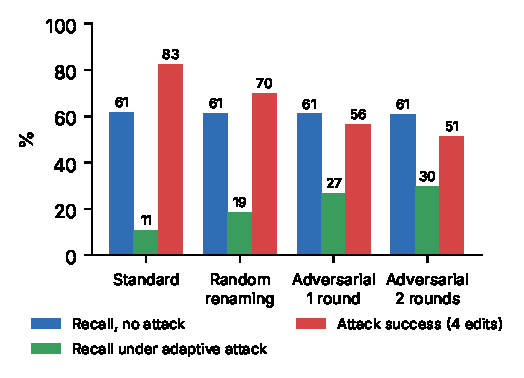
\includegraphics[width=\columnwidth]{defense.pdf}
\caption{Clean recall, recall under the adaptive attack, and attack success with four edits for each training method.}
\label{fig:defense}
\end{figure}

Adversarial training gives the largest gain. Two rounds cut four-edit evasion from 82.5\% to 51.3\% and nearly triple recall under attack, from 10.7\% to 29.7\%, while clean recall stays at about 61\% and false alarms stay at about 4.4\%. ROC AUC drops slightly, from 0.875 to 0.860. Random renaming helps less (69.8\% evasion), even though it covers the same edit types, which again shows that random perturbations are a poor proxy for a searching attacker. The second round adds less than the first, which suggests that further rounds would bring diminishing returns.

The defense also changes the attacker's strategy. Against the standard blend, TLD swaps were used 1,110 times by successful attacks; against the 2-round model they were used 433 times, and benign words (401) became almost as common. Adversarial hosts crafted against the standard model mostly stop working: only 25.7\% of them still evade the 2-round model. The attacker must search again, but a new search still succeeds for about half of the hosts.

\subsection{What does the defense cost?}

To measure side effects, we renamed 3,000 legitimate test hosts with two random edits using the test words, which mimics small or new legitimate sites with ordinary names. The standard blend flags 19.2\% of these renamed legitimate hosts. Adversarial training raises this to 22.1\% after one round and 28.0\% after two, and random renaming raises it to 38.2\%. The defense partly learns that unusual combinations of words and common TLDs are suspicious, which also hurts legitimate sites that look like them. Because the false alarm rate on real legitimate hosts is held at 5\%, this cost does not appear in standard metrics, so it should be reported separately.

\section{Discussion}

\textbf{Why host-only models are fragile.} A host-only detector judges a string that the attacker writes. The strongest signals it learns, such as cheap TLDs, digits and hyphens, are correlated with phishing because current operators choose them for cost and convenience, not because phishing requires them. Once operators adapt, these signals weaken. Adversarial training moves the model away from the cheapest signals, but it cannot create information that the host name does not contain.

\textbf{Recommendations.} For tools such as QR code scanners, we suggest: (i) treat a host-only score as a first filter and combine it with signals that are harder to rename, such as domain age, registration and certificate transparency data, and hosting reputation; (ii) avoid exposing raw scores, and rate-limit queries, since the attack needs about 34 queries per success; (iii) include adversarial training with an adaptive evaluation; and (iv) report robustness with a searching attacker and a held-out vocabulary, not only random perturbations.

\textbf{Limitations.} We do not check whether renamed domains are actually available for registration, so some may already be taken. Our edits and word lists are small, and the greedy attack is not optimal, so real attackers could do better. We assume a renamed host is as convincing to a victim as the original; a user study would be needed to confirm this, especially for edits such as appended words. Finally, we use one dataset and one model family, and other datasets may show different shortcuts.

\textbf{Ethics.} All hosts come from a public dataset of known phishing and legitimate URLs. We did not register any domains or contact any real systems.

\section{Conclusion}

Host-based phishing detectors are useful when a decision is needed before a page is opened, but they are easy to rename around. With a few dozen queries and up to four edits, an attacker evades a blended detector for 83.9\% of the phishing hosts it originally caught, and swapping to a common TLD alone succeeds 44.7\% of the time. Adversarial training lowers this to 51.3\% against an adaptive attacker and nearly triples recall under attack without hurting clean recall, but it flags more unusual legitimate names. Host-only scores should be one layer of defense, evaluated against attackers who search, not the whole defense.

\section*{Code and Data Availability}
The code, attack implementation and results are available at \url{https://github.com/aakashtiwarisolutions/name-games}. The PhiUSIIL dataset is available from the UCI Machine Learning Repository.

\begin{thebibliography}{99}

\bibitem{prasad2024phiusiil}
A.~Prasad and S.~Chandra, ``PhiUSIIL: A diverse security profile empowered phishing URL detection framework based on similarity index and incremental learning,'' \emph{Computers \& Security}, vol.~136, p.~103545, 2024.

\bibitem{ma2009beyond}
J.~Ma, L.~K. Saul, S.~Savage, and G.~M. Voelker, ``Beyond blacklists: Learning to detect malicious web sites from suspicious URLs,'' in \emph{Proc. ACM SIGKDD}, 2009, pp. 1245--1254.

\bibitem{sahoo2017survey}
D.~Sahoo, C.~Liu, and S.~C.~H. Hoi, ``Malicious URL detection using machine learning: A survey,'' \emph{arXiv:1701.07179}, 2017.

\bibitem{le2018urlnet}
H.~Le, Q.~Pham, D.~Sahoo, and S.~C.~H. Hoi, ``URLNet: Learning a URL representation with deep learning for malicious URL detection,'' \emph{arXiv:1802.03162}, 2018.

\bibitem{bahnsen2017rnn}
A.~C. Bahnsen, E.~C. Bohorquez, S.~Villegas, J.~Vargas, and F.~A. Gonz\'alez, ``Classifying phishing URLs using recurrent neural networks,'' in \emph{Proc. APWG Symposium on Electronic Crime Research (eCrime)}, 2017.

\bibitem{trad2025quishing}
F.~Trad and A.~Chehab, ``Detecting quishing attacks with machine learning techniques through QR code analysis,'' \emph{arXiv:2505.03451}, 2025.

\bibitem{arp2022dos}
D.~Arp, E.~Quiring, F.~Pendlebury, A.~Warnecke, F.~Pierazzi, C.~Wressnegger, L.~Cavallaro, and K.~Rieck, ``Dos and don'ts of machine learning in computer security,'' in \emph{Proc. USENIX Security Symposium}, 2022.

\bibitem{geirhos2020shortcut}
R.~Geirhos, J.-H. Jacobsen, C.~Michaelis, R.~Zemel, W.~Brendel, M.~Bethge, and F.~A. Wichmann, ``Shortcut learning in deep neural networks,'' \emph{Nature Machine Intelligence}, vol.~2, pp. 665--673, 2020.

\bibitem{goodfellow2015explaining}
I.~J. Goodfellow, J.~Shlens, and C.~Szegedy, ``Explaining and harnessing adversarial examples,'' in \emph{Proc. ICLR}, 2015.

\bibitem{biggio2018wild}
B.~Biggio and F.~Roli, ``Wild patterns: Ten years after the rise of adversarial machine learning,'' \emph{Pattern Recognition}, vol.~84, pp. 317--331, 2018.

\bibitem{madry2018towards}
A.~Madry, A.~Makelov, L.~Schmidt, D.~Tsipras, and A.~Vladu, ``Towards deep learning models resistant to adversarial attacks,'' in \emph{Proc. ICLR}, 2018.

\bibitem{pierazzi2020problemspace}
F.~Pierazzi, F.~Pendlebury, J.~Cortellazzi, and L.~Cavallaro, ``Intriguing properties of adversarial ML attacks in the problem space,'' in \emph{Proc. IEEE Symposium on Security and Privacy}, 2020.

\bibitem{apruzzese2023real}
G.~Apruzzese, H.~S. Anderson, S.~Dambra, D.~Freeman, F.~Pierazzi, and K.~Roundy, ``Real attackers don't compute gradients: Bridging the gap between adversarial ML research and practice,'' in \emph{Proc. IEEE Conference on Secure and Trustworthy Machine Learning (SaTML)}, 2023.

\bibitem{shirazi2019adversarial}
H.~Shirazi, B.~Bezawada, I.~Ray, and C.~Anderson, ``Adversarial sampling attacks against phishing detection,'' in \emph{Proc. IFIP Conference on Data and Applications Security and Privacy (DBSec)}, 2019.

\bibitem{aleroud2020bypassing}
A.~AlEroud and G.~Karabatis, ``Bypassing detection of URL-based phishing attacks using generative adversarial deep neural networks,'' in \emph{Proc. ACM International Workshop on Security and Privacy Analytics (IWSPA)}, 2020.

\bibitem{kintis2017combosquatting}
P.~Kintis, N.~Miramirkhani, C.~Lever, Y.~Chen, R.~Romero-G\'omez, N.~Pitropakis, N.~Nikiforakis, and M.~Antonakakis, ``Hiding in plain sight: A longitudinal study of combosquatting abuse,'' in \emph{Proc. ACM CCS}, 2017.

\bibitem{holgers2006homograph}
T.~Holgers, D.~E. Watson, and S.~D. Gribble, ``Cutting through the confusion: A measurement study of homograph attacks,'' in \emph{Proc. USENIX Annual Technical Conference}, 2006.

\bibitem{chen2016xgboost}
T.~Chen and C.~Guestrin, ``XGBoost: A scalable tree boosting system,'' in \emph{Proc. ACM SIGKDD}, 2016, pp. 785--794.

\end{thebibliography}

\end{document}
